\section{}
\label{sec:problem1}
%%%%%%%%%%%%%%%%%%%%%%%%%%%%%%%%%%%%%%%%%%%%%%%%%%%%%%%%%%%%%%%%%%%%%%
\paragraph{a)} Missing: relate cells and pines to nature.

\begin{figure}
    \centering
    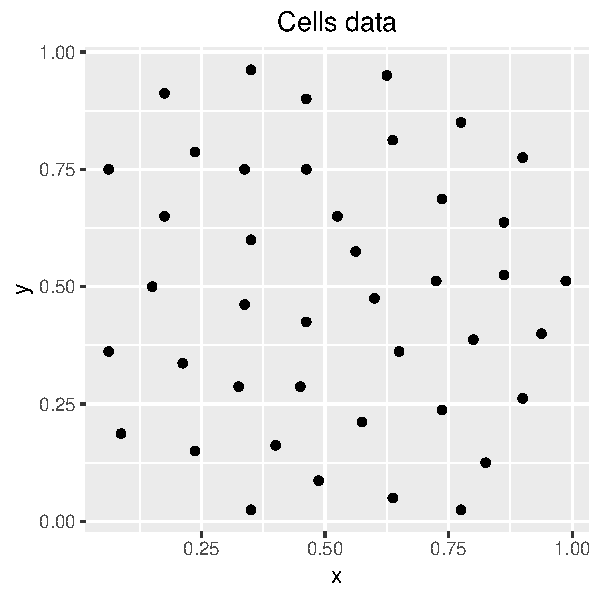
\includegraphics[scale=0.95]{figures/prob1_cells_points.pdf}
    \caption{Data points from \textit{cells.dat}}
    \label{fig:cells_points}
\end{figure}

\begin{figure}
    \centering
    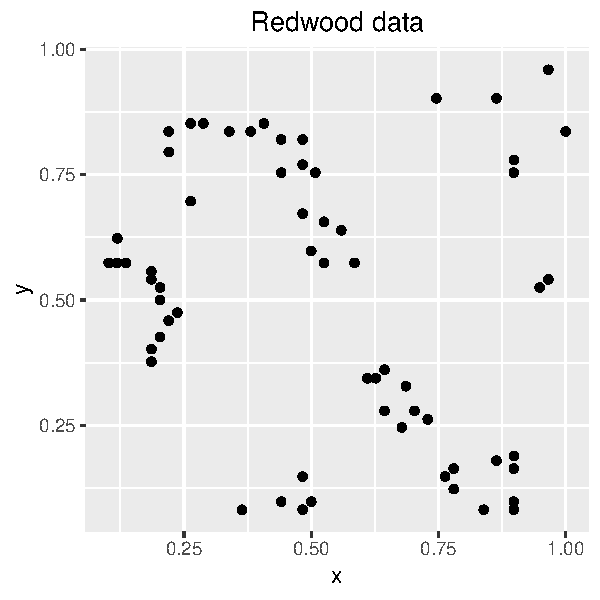
\includegraphics[scale=0.95]{figures/prob1_redwood_points.pdf}
    \caption{Data points from \textit{redwood.dat}}
    \label{fig:redwood_points}
\end{figure}

\begin{figure}
    \centering
    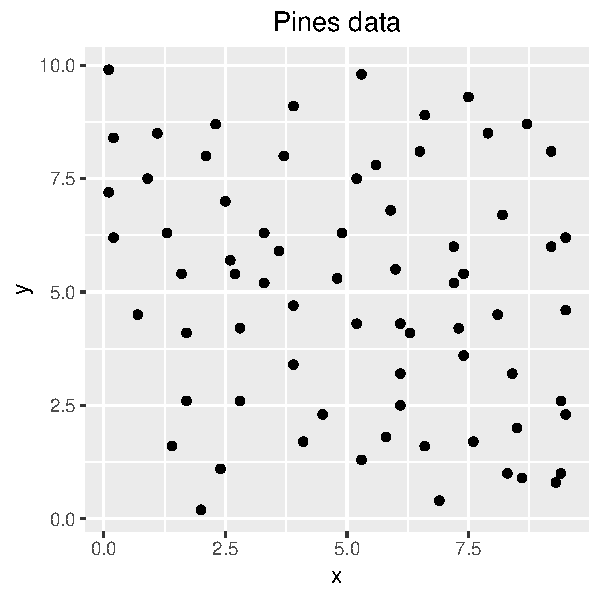
\includegraphics[scale=0.95]{figures/prob1_pines_points.pdf}
    \caption{Data points from \textit{pines.dat}}
    \label{fig:pines_points}
\end{figure}

Figures \ref{fig:cells_points}, \ref{fig:redwood_points} and \ref{fig:pines_points} show three different real data point patterns. These patterns have different properties. The pines data points in figure \ref{fig:pines_points} seem to be scattered around at random; some close together and some further away without any particular trend. The redwood data points (figure \ref{fig:redwood_points}) are more clustered. This is actually a known feature for redwood trees, as baby redwoods often grow on top of the roots of their parents to get nutrients (https://www.livescience.com/39461-sequoias-redwood-trees.html). The cells (figure \ref{fig:cells_points}) data on the other hand, show the exact opposite property. The points seem to be spread out to max out the space for each cell points, i.e. there seem to be a repulsive effect.

%%%%%%%%%%%%%%%%%%%%%%%%%%%%%%%%%%%%%%%%%%%%%%%%%%%%%%%%%%%%%%%%%%%%%%
\paragraph{b)} Missing: getting empirical functions that make any sense++.

$J(t)$ is an interaction function related to the distance from an event $\vect{x_0}$ to nearby events. Let $\textrm{B}_{x_0}(t)$ be the ball with center in $\vect{x_0}$ and radius $t \geq 0$. Then the number of events inside $\textrm{B}_{x_0}(t)$ is $k_{\textrm{B}_{x_0}(t)}$ and
\begin{equation}
    J(t) = \frac{\E{[k_{\textrm{B}_{x_0}(t)}-1]}}{|\textrm{B}_{x_0}(t) \cap \textrm{D}|}.
\end{equation}
The $-1$ corrects for the event $\vect{x_0}$ already known to be inside the ball. For a stationary Poisson Random Field, the expected number of events inside an subdomain of D is the intensity $\lambda_k$ times the area of the subdomain, since the intensity is constant over the whole domain. Thus, for a stationary Poisson RF, 
\begin{equation}
    J(t) = \frac{\lambda_k |\textrm{B}_{x_0}(t) \cap \textrm{D}|}{|\textrm{B}_{x_0}(t) \cap \textrm{D}|} = \lambda_k.
\end{equation}

Another alternative for evaluating the interaction is using the L-interactive function. For domains in $\R^2$, this is

\begin{equation}
    L(t) = \left[\frac{\E{[k_{\textrm{B}_{x_0}(t)}-1]}}{\lambda_k \pi}\right]^{1/2} = \left[\frac{J(t)|\textrm{B}_{x_0}(t) \cap \textrm{D}|}{\lambda_k \pi}\right]^{1/2}.
\end{equation}

Ignoring boundary effects, that is assuming $|\textrm{B}_{x_0}(t) \cap \textrm{D}| = |\textrm{B}_{x_0}(t)| = \pi t^2$, 
\begin{equation}
    L(t) = \left[\frac{J(t)\pi t^2}{\lambda_k \pi}\right]^{1/2} = \sqrt{\frac{J(t)}{\lambda_k}}t .
\end{equation}

Inserting for $J(t)$ we get that for stationary Poisson RF
\begin{equation}
    L(t) = t
\end{equation}

(Final conclusion:) It seems that a stationary Poisson model may be suitable for the pine tree data, but not for the two other data sets. The redwood data seem to be clustered and the cells data seem to be repulsive.

%%%%%%%%%%%%%%%%%%%%%%%%%%%%%%%%%%%%%%%%%%%%%%%%%%%%%%%%%%%%%%%%%%%%%%
\paragraph{c)}
We will now perform an empirical Monte Carlo test to assess whether a stationary Poisson Random Field is a suitable model for each point pattern. Assuming that the data is indeed from a stationary Poisson RF, and conditioning on the number of events, the locations of each event is independent and uniformly distributed in the domain.  
